% Sage Abstract Algebra Quick Reference
% (c) 2012 by Barry Balof, Thomas W.\ Judson, David Perkinson, Rao Potluri
% Licensed with the GNU Free Documentation License (GFDL)
%   http://www.gnu.org/copyleft/fdl.html
%
%  History
%
%    2012-06-15  Initial version based on Sage 5.0.1
%
%
\documentclass{article}
\usepackage{graphicx}  
\usepackage[landscape]{geometry}
\usepackage[pdftex]{color}
\usepackage{url}
\usepackage{multicol}
\usepackage{amsmath}
\usepackage{amsfonts}
\usepackage{textcomp}
\newcommand{\ex}{\color{blue}}
\newcommand{\apost}{\textquotesingle}
\newcommand{\warn}{\bf\color{red}}
\pagestyle{empty}
\advance\topmargin-.9in
\advance\textheight2in
\advance\textwidth3.0in
\advance\oddsidemargin-1.45in
\advance\evensidemargin-1.45in
\parindent0pt
\parskip2pt
% Section break, dictates column widths?
\newcommand{\hr}{\centerline{\rule{3.5in}{1pt}}}
% Adjust gap to affect spacing, page count
\newcommand{\sect}[1]{\hr\par\vspace*{2pt}\textbf{#1}\par}
% Mandatory indentation on subsidiary lines
\newcommand{\skipin}{\hspace*{12pt}}
% notation shortcut
\newcommand{\Z}{\mathbb{Z}}
\begin{document}
\begin{multicols*}{3}
\begin{center}
\textbf{Sage Quick Reference: Abstract Algebra}\\
B.\ Balof, T.\ W.\ Judson, D.\ Perkinson, R.\ Potluri\\
version 1.0, Sage Version 5.0.1\\
latest version: \url{http://wiki.sagemath.org/quickref}\\
GNU Free Document License, extend for your own use\\
Based on work by P.\ Jipsen, W.\ Stein, R.\ Beezer
\end{center}
% backup over center environment gap
\vspace{-2ex}
%*********************************************
\sect{Basic Help}
{\em com}$\langle$\verb!tab!$\rangle$\quad complete {\em command}\\
\verb!a.!$\langle$\verb!tab!$\rangle$\quad all methods for object \verb!a!\\
\verb!<command>?!\quad for summary and examples\\
\verb!<command>??!\quad for complete source code\\
\verb!*!{\em foo}\verb!*!?\quad list all commands containing {\em foo}\\
\verb!_!\quad underscore gives the previous output\\
\verb!www.sagemath.org/doc/reference!\quad  online reference\\
\verb!www.sagemath.org/doc/tutorial!\quad online tutorial\\
\verb!load foo.sage!\quad load commands from the file \verb!foo.sage!\\
\verb!attach foo.sage!\\
\skipin loads changes to \verb!foo.sage! automatically
\par
%
%*********************************************
\sect{Lists}
{\ex\verb!L = [2,17,3,17]!}\quad an ordered list\\
{\ex\verb!L[i]!}\quad the $i$th element of L\\
\skipin  {\warn Note: lists begin with the 0th element}\\
{\ex\verb!L.append(x)!}\quad adds $x$ to L\\
{\ex\verb!L.remove(x)!}\quad removes $x$ from L\\
{\ex\verb!L[i:j]!}\quad the $i$-th through $(j-1)$-th element of L\\
{\ex\verb!range(a)!}\quad list of integers from 0 to $a-1$ \\
{\ex\verb!range(a,b)!}\quad list of integers from $a$ to $b-1$\\
{\ex\verb![a..b]!}\quad list of integers from $a$ to $b$\\
{\ex\verb!range(a,b,c)!}\\
\skipin every $c$-th integer starting at $a$ and less than $b$\\
{\ex\verb!len(L)!}\quad length of L\\
{\ex\verb!M = [i^2 for i in range(13)]!}\\
\skipin list of squares of integers $0$ through $12$\\
{\ex\verb!N = [i^2 for i in range(13) if is_prime(i)]!}\\
\skipin list of squares of prime integers between $0$ and $12$\\
{\ex\verb!M + N!}\quad the concatenation of lists \verb!M! and \verb!N!\\
{\ex\verb!sorted(L)!}\quad a sorted version of \verb!L! (\verb!L! is not changed)\\
{\ex\verb!L.sort()!}\quad sorts \verb!L! (\verb!L! is changed)\\
{\ex\verb!set(L)!}\quad an unordered list of unique elements
\par
%*********************************************
\sect{Programming Examples}
Print the squares of the integers $0,\dots,14$:\\
{\ex\verb!for i in range(15):!}\\
{\ex\verb!     print i^2!}  \\

Print the squares of those integers in $\{0,\dots,14\}$ that are relatively prime to $15$:\\
{\ex\verb!for i in range(13):!}\\
{\ex\verb!     if gcd(i,15)==1:!}\\
 {\ex\verb!        print i^2!}

\par
%*********************************************
\sect{Preliminary Operations}
{\ex\verb!a = 3; b = 14!}\\
{\ex\verb!gcd(a,b) !}\quad greatest common divisor $a,b$\\
{\ex\verb!xgcd(a,b)!}\\
\skipin triple $(d,s,t)$ where $d=sa+tb$ and $d=\gcd(a,b)$\\
{\ex\verb!next_prime(a)!}\quad  next prime after $a$\\
{\ex\verb!previous_prime(a)!}\quad  prime before $a$\\
{\ex\verb!prime_range(a,b)!}\quad primes $p$ such that $a\leq p<b$\\
{\ex\verb!is_prime(a)!}\quad is \verb!a! prime?\\
{\ex\verb!b % a!} the remainder of $b$ upon division by $a$\\
{\ex\verb!a.divides(b)!}\quad does $a$ divide $b$?
\par
%*********************************************
\sect{Group Constructions}
{\warn Permutation multiplication is left-to-right.}\\
{\ex\verb!G = PermutationGroup([[(1,2,3),(4,5)],[(3,4)]])!}\\
\skipin perm.\ group with generators $(1,2,3)(4,5)$ and $(3,4)$\\
{\ex\verb!G = PermutationGroup(["(1,2,3)(4,5)","(3,4)"])!}\\
\skipin alternative syntax for defining a permutation group
{\ex\verb!S = SymmetricGroup(4)!}\quad the symmetric group, $S_4$\\
{\ex\verb!A = AlternatingGroup(4)!}\quad alternating group, $A_4$\\
{\ex\verb!D = DihedralGroup(5)!}\quad dihedral group of order $10$\\
{\ex\verb!Ab = AbelianGroup([0,2,6])!}\quad the group $\Z\times\Z_2\times\Z_6$\\
{\ex\verb!Ab.0, Ab.1, Ab.2!}\quad the generators of \verb!Ab!\\
{\ex\verb!a,b,c = Ab.gens()!}\\
\skipin shorthand for \verb!a = Ab.0; b = Ab.1; c = Ab.2!\\
{\ex\verb!C = CyclicPermutationGroup(5)!}\\
{\ex\verb!Integers(8)!}\quad the group $\Z_8$\\
{\ex\verb!GL(3,QQ)!}\quad general linear group of $3\times3$ matrices\\
{\ex\verb!m = matrix(QQ,[[1,2],[3,4]])!}\\
{\ex\verb!n = matrix(QQ,[[0,1],[1,0]])!}\\
{\ex\verb!MatrixGroup([m,n])!}\\
\skipin the (infinite) matrix group with generators \verb!m! and \verb!n!\\
{\ex\verb!u = S([(1,2),(3,4)])!};\quad{\ex\verb!v = S((2,3,4))!} elements of \verb!S!
{\ex\verb!S.subgroup([u,v])!}\\
\skipin the subgroup of \verb!S! generated by \verb!u! and \verb!v!\\
{\ex\verb!S.quotient(A)!}\quad the quotient group \verb!S/A!\\
{\ex\verb!A.cartesian_product(D)!}\quad the group \verb'A'$\times$\verb!D!\\
{\ex\verb!A.intersection(D)!}\quad the intersection of groups \verb'A' and \verb!D!\\
{\ex\verb!D.conjugate(v)!}\quad the group \verb!v!$^{-1}$\verb!Dv!\\
{\ex\verb!S.sylow_subgroup(2)!}\quad a Sylow $2$-subgroup of \verb!S!\\
{\ex\verb!D.center()!}\quad the center of \verb!D!\\
{\ex\verb!S.centralizer(u)!}\quad the centralizer of \verb!x! in \verb!S!\\
{\ex\verb!S.centralizer(D)!}\quad the centralizer of \verb!D! in \verb!S!\\
{\ex\verb!S.normalizer(u)!}\quad the normalizer of \verb!x! in \verb!S!\\
{\ex\verb!S.normalizer(D)!}\quad the normalizer of \verb!D! in \verb!S!\\
{\ex\verb!S.stabilizer(3)!}\quad subgroup of \verb!S! fixing $3$
\par
%*********************************************
% TODO
% homomorphisms
% cyclic permutation groups
% additive abelian group
% multiplicative abelian group
% group actions
% conjugacy classes
\sect{Group Operations}
{\ex\verb!S = SymmetricGroup(4); A = AlternatingGroup(4)!}\\
{\ex\verb!S.order()!}\quad the number of elements of \verb!S!\\
{\ex\verb!S.gens()!}\quad generators of \verb!S!\\
{\ex\verb!S.list()!}\quad the elements of \verb!S!\\
{\ex\verb!S.random_element()!}\quad a random element of \verb!S!\\
{\ex\verb!u*v!}\quad the product of elements \verb!u! and \verb!v! of \verb!S!\\
{\ex\verb!v^(-1)*u^3*v!}\quad the element \verb!v!$^{-1}$\verb!u!$^3$\verb!v! of \verb!S!\\
{\ex\verb!u.order()!}\quad the order of \verb!u!\\
{\ex\verb!S.subgroups()!}\quad the subgroups of \verb!S!\\
{\ex\verb!S.normal_subgroups()!}\quad the normal subgroups of \verb!S!\\
{\ex\verb!A.cayley_table()!}\quad the multiplication table for \verb!A!\\
{\ex\verb!u in S!}\quad is \verb!u! an element of \verb!S!?\\
{\ex\verb!u.word_problem(S.gens())!}\\
\skipin write \verb!u! as a product of the generators of \verb!S!\\
{\ex\verb!A.is_abelian()!}\quad is \verb!A! abelian?\\
{\ex\verb!A.is_cyclic()!}\quad is \verb!A! cyclic?\\
{\ex\verb!A.is_simple()!}\quad is \verb!A! simple?\\
{\ex\verb!A.is_transitive()!}\quad is \verb!A! transitive?\\
{\ex\verb!A.is_subgroup(S)!}\quad is \verb!A! a subgroup of \verb!S!?\\
{\ex\verb!A.is_normal(S)!}\quad is \verb!A! a normal subgroup of \verb!S!?\\
{\ex\verb!S.cosets(A)!}\quad the right cosets of \verb!A! in \verb!S!\\
{\ex\verb!S.cosets(A,!\apost\verb!left!\apost\verb!)!}\quad the left cosets of \verb!A! in \verb!S!
{\ex\verb!g = S.cayley_graph()!}\quad Cayley graph of \verb!S!\\
{\ex\verb!g.show3d(color_by_label=True, edge_size=0.01,!}\\
\skipin{\ex\verb!vertex_size=0.03)!} see below:\\
\begin{center}
  \vskip-0.1in
  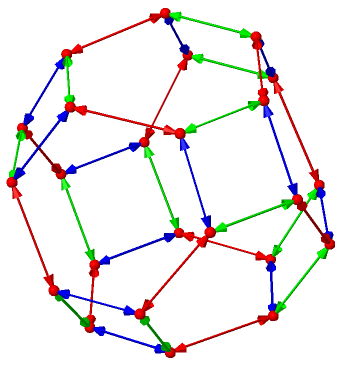
\includegraphics[width=1.5in]{cayley.png}
\end{center}
\vskip-0.1in
\par
%*********************************************
\pagebreak
\sect{Ring and Field Constructions}

{\ex\verb!ZZ!}
\quad integral domain of integers, ${\mathbb Z}$\\
{\ex\verb!Integers(7)!}
\quad ring of integers mod 7, ${\mathbb Z}_7$\\
{\ex\verb!QQ!}
\quad field of rational numbers, ${\mathbb Q}$\\
{\ex\verb!RR!}
\quad field of real numbers, ${\mathbb R}$\\
{\ex\verb!CC!}
\quad field of complex numbers, ${\mathbb C}$\\
{\ex\verb!RDF!}\quad real double field, inexact\\
{\ex\verb!CDF!}\quad complex double field, inexact\\
{\ex\verb!RR!}\quad 53-bit reals, inexact, not same as {\ex\verb!RDF!}\\
{\ex\verb!RealField(400)!}\quad 400-bit reals, inexact\\
{\ex\verb!ComplexField(400)!}\quad complexes, too\\
{\ex\verb!ZZ[I]!}\quad the ring of Gaussian integers\\
{\ex\verb!QuadraticField(7)!} 
\quad the quadratic field, ${\mathbb Q}(\sqrt{7}\,)$\\
{\ex\verb!CyclotomicField(7)!}\\
\skipin smallest field containing $\mathbb{Q}$ and the zeros of $x^7-1$\\
{\ex\verb!AA,  QQbar!} 
\quad field of algebraic numbers, $\overline{\mathbb Q}$\\
{\ex\verb!FiniteField(7)!}\quad the field $\mathbb Z_7$\\
{\ex\verb!F.<a> = FiniteField(7^3)!}\\
\skipin finite field in $a$ of size $7^3$,  ${\rm GF}(7^3)$\\
{\ex\verb!SR!}\quad ring of symbolic expressions\\
{\ex\verb!M.<a>=QQ[sqrt(3)]!}\quad the field $\mathbb{Q}[\sqrt{3}]$, with $a=\sqrt{3}$.\\
{\ex\verb!A.<a,b>=QQ[sqrt(3),sqrt(5)]!}\\
\skipin the field $\mathbb{Q}[\sqrt{3},\sqrt{5}]$ with $a=\sqrt{3}$ and $b=\sqrt{5}$.
{\ex\verb!z = polygen(QQ,!\apost\verb!z!\apost\verb!); K = NumberField(x^2 - 2,!\apost\verb!s!\apost\verb!)!}\\
\skipin the number field in $s$ with defining polynomial $x^2-2$\\
{\ex\verb!s = K.0!}\quad set \verb!s! equal to the generator of \verb!K!\\
{\ex\verb!D = ZZ[sqrt(3)]!}\\
{\ex\verb!D.fraction_field()!}\\
\skipin field of fractions for the integral domain \verb!D!
\par
%*********************************************
\sect{Ring Operations}
{\warn Note: Operations may depend on the ring}\\
{\ex\verb!A = ZZ[I]; D = ZZ[sqrt(3)]!}\quad some rings\\
{\ex\verb!A.is_ring()!}\quad is $A$ a ring? \\
{\ex\verb!A.is_field()!}\quad is $A$ a field?\\
{\ex\verb!A.is_commutative()!}\quad is $A$ commutative?\\
{\ex\verb!A.is_integral_domain()!}\\
\skipin \verb!True! is $A$ an integral domain?\\
{\ex\verb!A.is_finite()!}\quad is $A$ is finite?\\
{\ex\verb!A.is_subring(D)!}\quad is $A$ a subring of $D$?\\
{\ex\verb!A.order()!}\quad the number of elements of $A$\\
{\ex\verb!A.characteristic()!}\quad the characteristic of $A$\\
{\ex\verb!A.zero()!}\quad the additive identity of $A$\\
{\ex\verb!A.one()!}\quad the multiplicative identity of $A$\\
{\ex\verb!A.is_exact()!}\\
\skipin \verb!False! if \verb!A! uses a floating point representation\\
{\ex\verb!a, b = D.gens(); r = a + b!}\\
{\ex\verb!r.parent()!}\quad the parent ring of $r$ (in this case, \verb!D!)\\
{\ex\verb!r.is_unit()!}\quad is $r$ a unit?
\par
%*********************************************
\sect{Polynomials}

{\ex\verb!R.<x> = ZZ[ ]!}\quad \verb!R! is the polynomial ring $\mathbb Z[x]$\\
{\ex\verb!R.<x> = QQ[ ]; R = PolynomialRing(QQ,!\apost\verb!x!\apost\verb!); R = QQ[!\apost\verb!x!\apost\verb!]!}\\
\skipin \verb!R! is the polynomial ring  $\mathbb Q[x]$ \\
{\ex\verb!S.<z> = Integers(8)[ ]!}\quad \verb!S! is the polynomial ring  $\mathbb Z_8[z]$\\
{\ex\verb!S.<s, t> = QQ[ ]!}\quad \verb!S! is the polynomial ring $\mathbb Q[s, t]$\\
{\ex\verb!p = 4*x^3 + 8*x^2 - 20*x - 24!}\\
\skipin a polynomial in \verb!R!  ($=\mathbb{Q}[x]$)\\
{\ex\verb!p.is_irreducible()!}\quad is $p$ irreducible over  $\mathbb Q[x]$?\\
{\ex\verb!q = p.factor()!}\quad factor $p$  \\
{\ex\verb!q.expand()!}\quad expand \verb!q!\\
{\ex\verb!p.subs(x=3)!}\quad evaluates $p$ at $x=3$ \\
{\ex\verb!R.ideal(p)!}\quad the ideal in $R$ generated by $p$ \\
{\ex\verb!R.cyclotomic_polynomial(7)!}\\
\skipin the cyclotomic polynomial $x^6 + x^5 + x^4 + x^3 + x^2 + x + 1$ \\
{\ex\verb!q = x^2-1!}\\
{\ex\verb!p.divides(q)!}\quad  does $p$ divide $q$?\\
{\ex\verb!p.quo_rem(q)!}\\
\skipin the quotient and remainder of \verb!p! upon division by \verb!q!\\
{\ex\verb!gcd(p, q)!}\quad the greatest common divisor of $p$ and $q$\\
{\ex\verb!p.xgcd(q)!}\quad the extended gcd of $p$ and $q$ \\
{\ex\verb!I = S.ideal([s*t+2,s^3-t^2])!}\\
\skipin the ideal $(st+2,s^3-t^2)$ in \verb!S!  ($=\mathbb{Q}[s,t])$)\\
{\ex\verb!S.quotient(I)!}\quad the quotient ring, $S/I$\\
\par
%*********************************************
\sect{Field Operations}
{\ex\verb!A.<a,b>=QQ[sqrt(3),sqrt(5)]!}\\
{\ex\verb!C.<c> = A.absolute_field()!}\\
\skipin ``flattens'' a relative field extension\\
{\ex\verb!A.relative_degree()!}\\
\skipin the degree of the relative extension field\\
{\ex\verb!A.absolute_degree()!}\\
\skipin the degree of the absolute extension\\
{\ex r = a + b; \verb!r.minpoly()!}\\
\skipin the minimal polynomial of the field element \verb!r!
{\ex\verb!C.is_galois()!}\quad is \verb!C! a Galois extension of $Q$?\\
\par
%*********************************************
\end{multicols*}

\end{document}
